\section{Additional Regression Techniques}
\label{app:adtl_regression}
\nocite{neu_ModelSynth}
\nocite{cuth_regression}
\nocite{bbc_chebyshev}

% Run /scripts/appendix/powerSeries.m
\begin{figure}[ht!]
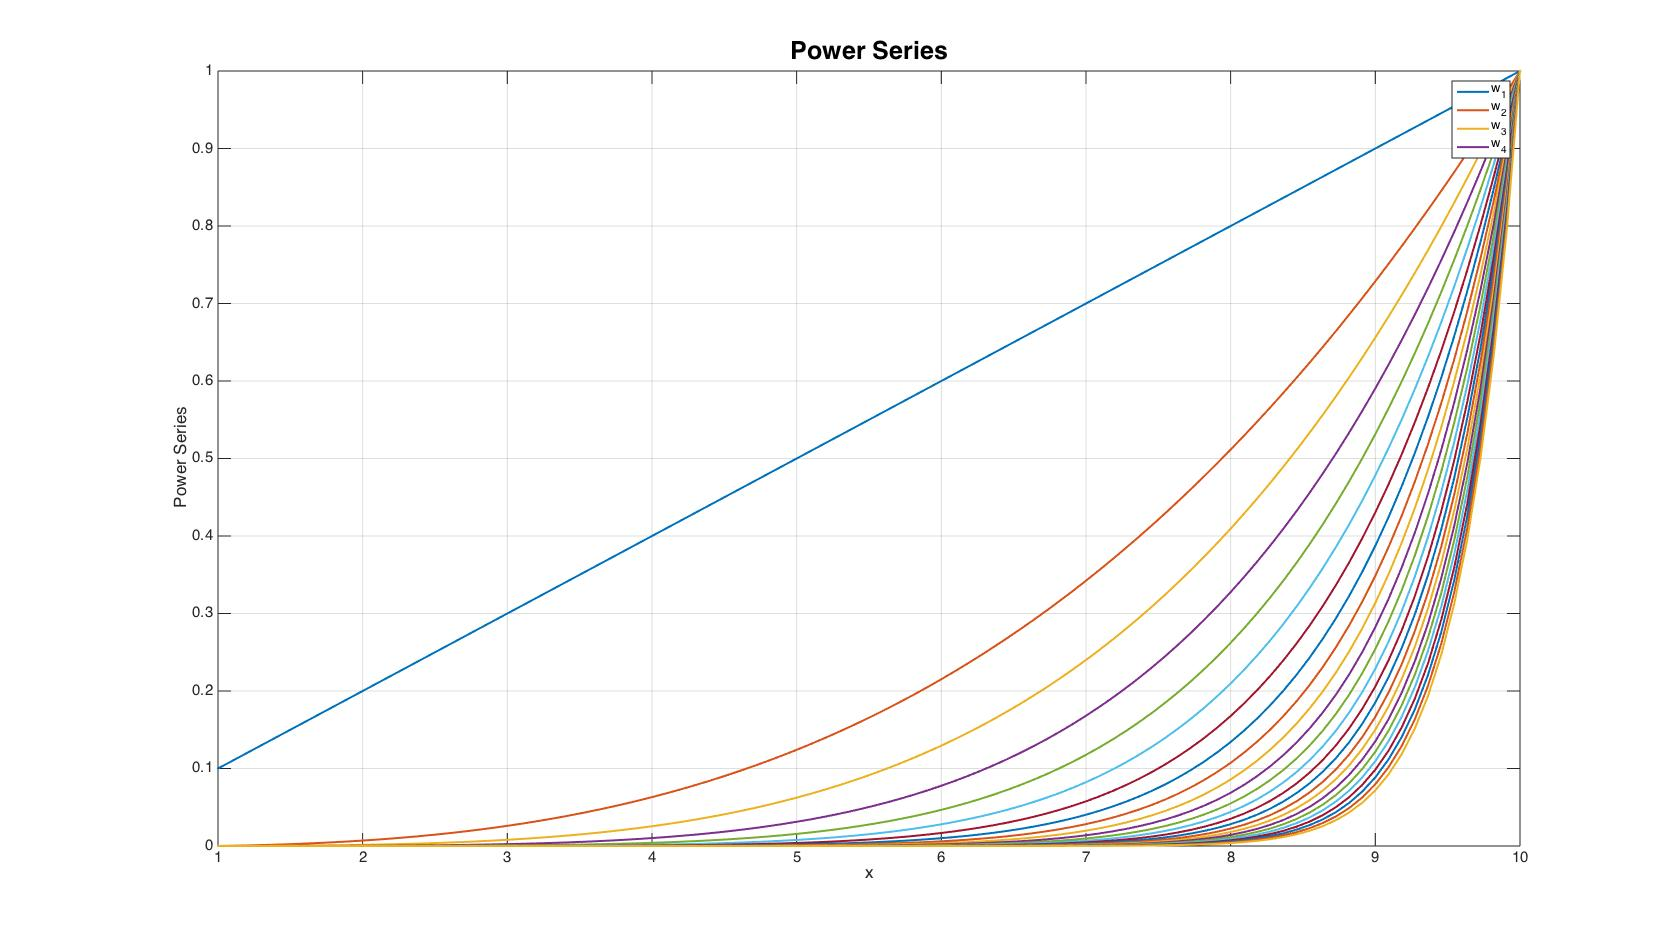
\includegraphics[keepaspectratio=true,width=6in]{./figures/appendix/powerSeries.jpg}
\centering
\caption{Power Series \cite{beyene_uwave}[Fig: 1]}
\label{fig:powerSeries}
\end{figure}



This section will cover the theory behind a computational method that should improve the results obtained in Section: \ref{sec:regression}. As previously stated, the main problem with applying Levy's approach to capacitor modeling is that it is ill-suited for wide bandwidth applications. As stated by Beyene, ``this is because the ordinary power series ${\omega ^0, \omega ^1, \omega ^2, \omega ^3,...}$ have a large dynamic range, and they become almost parallel at higher orders. As show in Figure: \ref{fig:powerSeries}, for higher orders, the shapes of the power series become very similar over most of the normalized frequency range. \cite{beyene_uwave}''

\begin{equation}
\label{equ:cheby}
T_{n+1} = 2xT_{n}-T_{n-1}
\end{equation}

\begin{equation}
    \label{equ:chebyPolys}
    \begin{split}
         T_0(x) &= 1           \\
         T_1(x) &= x           \\
         T_2(x) &= 2x^2-1      \\
         T_3(x) &= 4x^3-3x     \\
         T_4(x) &= 8x^4-8x^2+1 \\
         T_5(x) &= 16x^5-20x^3+5x
    \end{split}
\end{equation}

The proposed methodology uses Chebyshev polynomials of the first kind to circumvent this problem. As seen in Equation: \eqref{equ:cheby}, they are recursively defined with $T_0 = 1$ and $T_1 = x$. This results in polynomials that are orthogonal over a normalized frequency range, as seen in Figure: \ref{fig:cheby}. Gao\cite{gao_blackBox} shows that the frequency terms in an LSE can be replaced with Chebyshev polynomials. The coefficients found via this method are not the same as the coefficients in the frequency space. One needs to use Clenshaw's Recurrence Formula \cite{gao_blackBox}[Equation: 11] in order to get the desired coefficients. This method should produce a result that is more accurate due to its avoidance of the ill-conditioned matrix while solving the system of equations.

% Run /scripts/appendix/cheby.m
\begin{figure}[ht!]
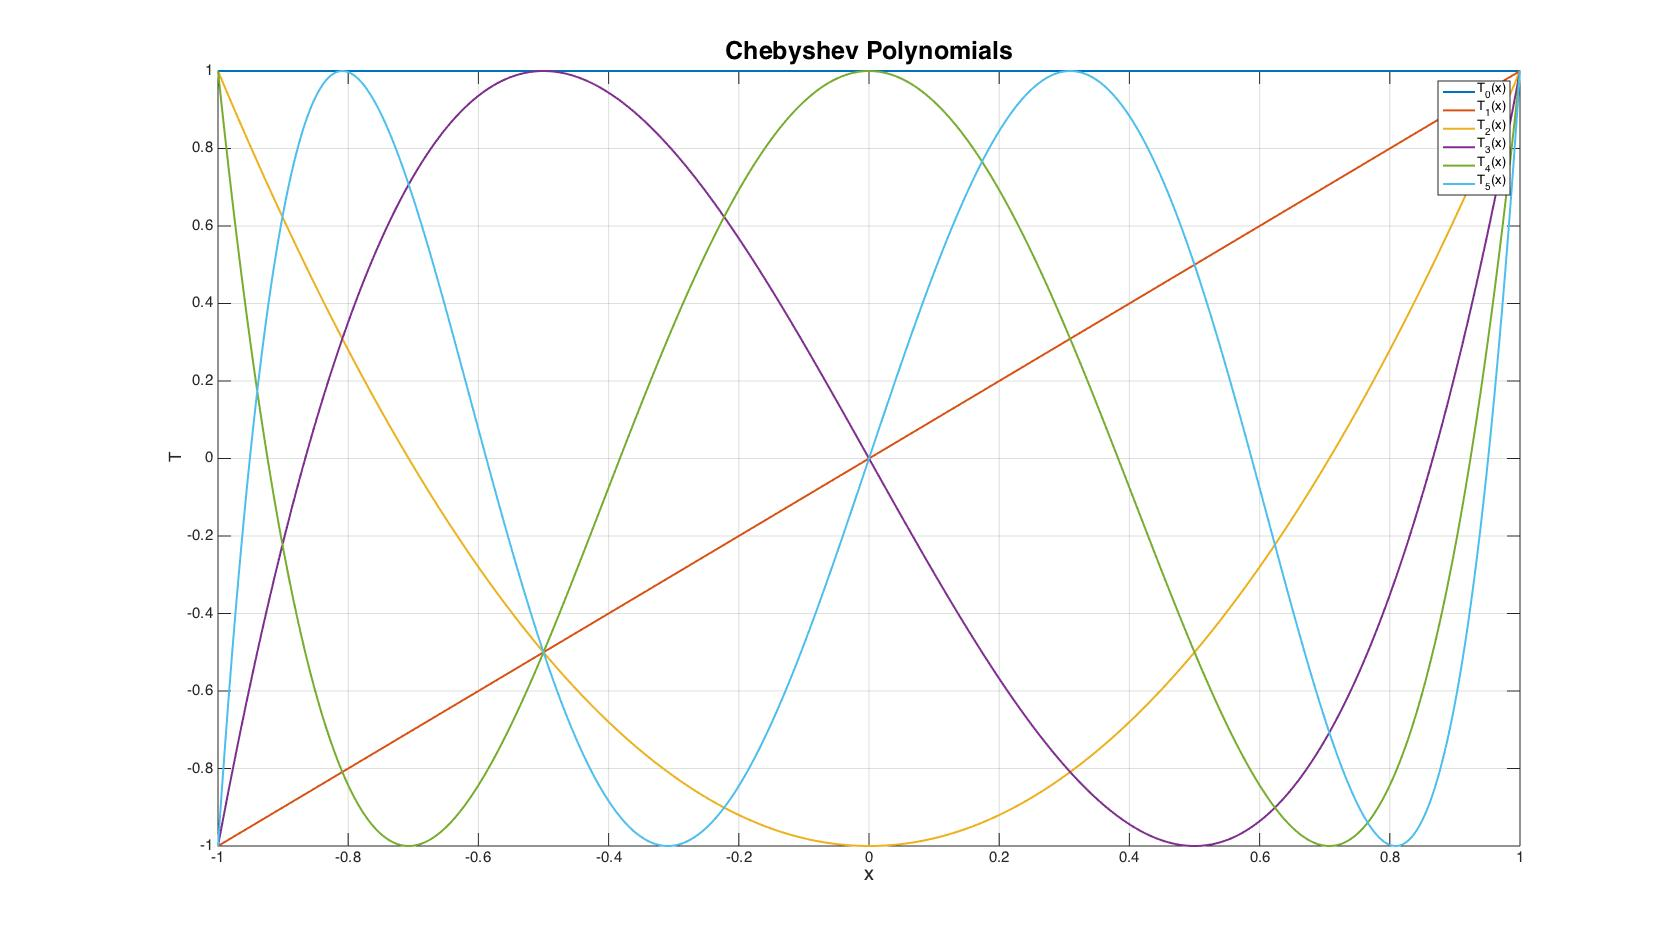
\includegraphics[keepaspectratio=true,width=6in]{./figures/appendix/cheby.jpg}
\centering
\caption{Chebyshev Polynomials \cite{wolf_cheby}}
\label{fig:cheby}
\end{figure}



